\documentclass[11pt]{article}

% --- packages -------------------------------------------------------------
\usepackage[T1]{fontenc}
\usepackage[utf8]{inputenc}
\usepackage{lmodern}
\usepackage[a4paper,margin=1in]{geometry}
\usepackage{microtype}
\usepackage{amsmath,amssymb}
\usepackage{booktabs}
\usepackage{graphicx}
\usepackage{caption}
\usepackage{enumitem}
\usepackage{siunitx}
\usepackage{xcolor}
\usepackage{titlesec}
\usepackage[hidelinks]{hyperref}

% --- style ----------------------------------------------------------------
\definecolor{vblue}{HTML}{1F4E79}
\hypersetup{colorlinks=true, linkcolor=vblue, urlcolor=vblue, citecolor=vblue}
\titleformat{\section}{\large\bfseries\color{vblue}}{\thesection}{0.6em}{}
\titleformat{\subsection}{\normalsize\bfseries}{\thesubsection}{0.6em}{}
\captionsetup{font=small,labelfont=bf,labelsep=period}
\setlist{itemsep=2pt,topsep=3pt,parsep=0pt}
\sisetup{detect-all,group-minimum-digits=4}

% A visible TODO marker for anything not in the source of truth.
\newcommand{\todo}[1]{\textcolor{red}{\textbf{[TODO: #1]}}}

% Shorthands for the engine's named quantities.
\newcommand{\Cllr}{C_{\mathrm{llr}}}
\newcommand{\Cllrmin}{C_{\mathrm{llr}}^{\min}}
\newcommand{\diagmean}{\texttt{diag\_mean}}
\newcommand{\diagcontrast}{\texttt{diag\_contrast}}
\newcommand{\code}[1]{\texttt{#1}}

\title{\vspace{-1.2cm}\textbf{Verity}\\[2pt]
\large A Calibrated, Auditable Deployment Layer for Forensic Surface Comparison}
\author{Eric Hare\\[-2pt]\small \href{mailto:ericrhare@gmail.com}{ericrhare@gmail.com}}
\date{\small June 2026 \;\textbar\; Technical White Paper}

\begin{document}
\maketitle
\vspace{-0.6cm}

% ==========================================================================
\begin{abstract}
\noindent
Two decades of community review --- the National Research Council's 2009 report
and the 2016 PCAST report --- found that the feature-comparison forensic
disciplines, firearms and toolmark identification among them, lack characterized
error rates. Cuellar et al.\ (2024) sharpened the point: \emph{no} black-box study
of firearm comparison has yet properly characterized one. Verity does not claim to
supply the missing universal error rate; we argue no single number exists. Instead
it operationalizes the response a statistician would give: report a \emph{calibrated
weight of evidence} --- a likelihood ratio (LR) --- with a \emph{characterized
cost} ($\Cllr$) on a \emph{named} reference population, and refuse to emit an LR
outside the domain on which it was validated.

Verity is, deliberately, not a new matching algorithm. It is the production,
deployment, and calibration layer for the CSAFE / Iowa State research program
(Hare, Hofmann \& Carriquiry 2017) and the NIST congruent-matching line
(Song 2013; Song et al.\ 2018). Its contributions are five: (1) \emph{unification}
--- one calibrated pipeline that scores striated, impressed, and fractured marks
through \emph{Congruent Matching Regions} (CMR), a dimension-agnostic
generalization of Song's Congruent Matching Cells; (2) a calibrated-LR-with-honest-scope
answer to Cuellar et al.; (3) a glass-box decision layer --- region-level
attribution plus a monotone, bounded calibration we call an \emph{audit firewall};
(4) production engineering --- a native Rust X3P codec, language bindings, and a
deployed calibrated-LR API; and (5) a small methodological result --- a
\diagcontrast{} scorer, selected over the Phase-1 mean-diagonal score and over
multivariate fusion \emph{by data, not assumption}. On the Hamby-252 bullet
benchmark Verity attains a barrel-disjoint (source-disjoint) test
$\Cllr = \num{0.113} \pm \num{0.066}$ with test AUC $\num{1.000}$; we report
validation results per study and never pool across firearm makes. Beyond bullets,
the \emph{same} pipeline under \emph{one} scorer configuration is validated
source-disjoint on impressed cartridge breech faces (Fadul) and striated
screwdriver toolmarks (\code{tmaRks}), where CMR instantiates the counting
principles of Song's Congruent Matching Cells and of the Chumbley statistic and
approaches each specialist's performance --- one calibrated algorithm, three
reductions, each \emph{measured} rather than asserted.
\end{abstract}

% ==========================================================================
\section{Introduction: a discipline without a characterized error rate}
\label{sec:intro}

Firearm and toolmark identification asks whether two marked surfaces --- two
bullets, two cartridge cases, two toolmarks --- were produced by the same source.
For most of its history the answer has rested on a trained examiner's holistic
judgement of ``sufficient agreement.'' The 2009 National Research Council report
\emph{Strengthening Forensic Science in the United States}~\cite{nrc2009} found that
the pattern-comparison disciplines had not been shown, with the rigor of
measurement science, to do what they claim. The 2016 report of the President's
Council of Advisors on Science and Technology (PCAST)~\cite{pcast2016} made the
requirement explicit: a feature-comparison method is \emph{foundationally valid}
only if it has been empirically tested on appropriate samples and has a
\emph{characterized error rate}.

Cuellar, Vanderplas, Luby \& Rosenblum (2024)~\cite{cuellar2024} examined the
black-box studies offered in response and concluded that \emph{every one} of them
has methodological problems severe enough that none establishes an error rate one
could responsibly carry into court: inappropriate sampling, set-based designs that
leak class information, inconclusives handled in ways that flatter the method, and
--- most relevant here --- error rates reported as if they were properties of the
\emph{discipline} rather than of a particular study population.

Verity takes a deliberately narrower and, we argue, more honest stance. There is
no single ``error rate of firearms identification,'' because the answer depends on
the firearm population, the manufacturing process, the wear state, and the scan
quality. What \emph{can} be reported, defensibly, is:

\begin{enumerate}
  \item a \textbf{likelihood ratio} --- how much more probable the observed surface
        agreement is if the two marks share a source than if they do not --- which
        is prior-independent and is the form of evidence the courts and the
        forensic-statistics literature ask for;
  \item the \textbf{calibration cost} $\Cllr$~\cite{brummer2006} of the system that
        produced that LR, measured \emph{on a named reference population} under a
        \emph{source-disjoint} protocol, so the number means ``how well this system
        is calibrated on data like this,'' not ``how often examiners are wrong'';
  \item an explicit \textbf{scope}: outside the validated domain, Verity declines to
        emit an LR rather than extrapolate.
\end{enumerate}

This is the same move that forensic speaker comparison made years ago, and it is
why Verity borrows that field's evaluation machinery. The remainder of this paper
describes the lineage Verity builds on (\S\ref{sec:lineage}), the comparison
method and its cross-modality generalization (\S\ref{sec:method}), the calibration
firewall that turns a score into evidence (\S\ref{sec:calibration}), the
source-disjoint validation that answers Cuellar et al.\ directly
(\S\ref{sec:validation}), the limitations we are candid about (\S\ref{sec:limits}),
and the open platform on which all of this runs (\S\ref{sec:platform}).

% ==========================================================================
\section{Lineage and contribution}
\label{sec:lineage}

Verity is downstream of, and indebted to, a specific body of work; naming it
precisely is part of being honest about what is and is not new here.

\paragraph{What Verity builds on.}
The automatic comparison of bullet land impressions is the CSAFE / Iowa State
method of Hare, Hofmann \& Carriquiry~\cite{hare2017}: striation signatures are
extracted from each land, compared on \emph{multiple} features (cross-correlation
among them, alongside matching/non-matching striae counts and related measures),
and combined by a trained random forest --- that paper is explicit that
cross-correlation alone does not suffice. The open \code{bulletxtrctr} pipeline
and the three-similarity-score study of Vanderplas et al.~\cite{vanderplas2020}
are the reference implementation and benchmark; Verity's Phase-1 score adopts the
signature-extraction-and-correlation front end of that line. The cell-counting idea
for impressed marks
--- partition one surface into cells, register each against the other, and count
the cells whose best-fit translations and rotations agree --- is Song's Congruent
Matching Cells (CMC)~\cite{song2013} and the NIST error-rate line built on
it~\cite{song2018}, with \code{cmcR} as the open reference
implementation~\cite{zemmels2023}. The objective comparison of striated toolmarks by a
distribution-free statistic is Chumbley et al.~\cite{chumbley2010}, improved and
made deterministic by Hadler \& Morris (the \code{toolmaRk}
package)~\cite{hadler2018} and adapted to bullet lands by Krishnan \&
Hofmann~\cite{krishnan2019}; open, fully automatic cartridge-case comparison is
also due to Tai \& Eddy~\cite{tai2018}. The surface
representation is the ISO~25178-72 X3P format, for which the reference reader is the
\code{x3ptools} R package~\cite{x3ptools2024}. The evaluation metric $\Cllr$ and the
calibration philosophy come from forensic speaker recognition, originally
Br\"ummer \& du Preez~\cite{brummer2006}, with logistic-regression calibration as
codified for forensic use by Morrison~\cite{morrison2013} and the validation
regime for LR methods set out by Meuwly, Ramos \& Haraksim~\cite{meuwly2017}.

\paragraph{What is novel in Verity.} Five things, and we state them plainly so the
boundary is clear:
\begin{enumerate}
  \item \textbf{Unification.} One calibrated pipeline scores striated, impressed,
        and (in principle) fractured marks through \emph{Congruent Matching Regions}
        (\S\ref{sec:cmr}), a generalization of CMC from 2-D cells under
        translation+rotation to regions of any dimension under any transformation
        group. CMC and the 1-D Chumbley statistic become two instantiations of one
        algorithm --- and we \emph{demonstrate} both reductions source-disjoint, under
        a single scorer configuration, alongside bullets (\S\ref{sec:crossmodal}); the
        3-D fractured case is the general form, not yet validated.
  \item \textbf{A calibrated-LR answer to Cuellar et al.} Rather than a single
        disputed error rate, Verity reports a bounded LR with a per-study,
        source-disjoint $\Cllr$ (\S\ref{sec:validation}).
  \item \textbf{A glass-box decision layer.} Region-level attribution (which parts
        of the surface drove the match) plus a \emph{monotone, bounded} calibration
        --- the ``audit firewall'' (\S\ref{sec:calibration}) --- so the reported
        evidence is interpretable regardless of how the underlying score was
        produced.
  \item \textbf{Production engineering.} A native Rust X3P codec, Python and R
        bindings, a deployed calibrated-LR REST API, and a data catalog
        (\S\ref{sec:platform}).
  \item \textbf{A small methodological result.} The \diagcontrast{} scorer
        (\S\ref{sec:aggregate}), selected over the mean-diagonal baseline and over
        multivariate fusion by a barrel-disjoint ablation (\S\ref{sec:scorerablation}).
\end{enumerate}

\noindent
Verity is the \emph{deployment, calibration, and validation layer} for this research
program --- not a claim to have invented the comparison.

% ==========================================================================
\section{Method}
\label{sec:method}

The pipeline is four stages: surface metrology, region extraction, pairwise
comparison, and aggregation. We describe the striated (bullet-land) path in full
because it is the one we validate most heavily, then give the cross-modality
generalization.

\subsection{Surface metrology}
\label{sec:metrology}
A raw X3P scan is a height field $z(x,y)$ on a regular grid with invalid (masked)
points. Individualizing texture lives in a narrow band of spatial wavelengths;
everything coarser is the shape of the object and everything finer is measurement
noise. Verity isolates the band with the standard ISO operations:

\begin{enumerate}
  \item \textbf{Form removal} (the ISO~25178 F-operation). Fit a least-squares 2-D
        polynomial of total degree~2 to the valid points and subtract it, removing
        gross shape such as the curvature of a bullet land. With coordinates
        normalized to $[-1,1]$ the design uses the monomials $x^i y^j,\ i+j\le 2$.
  \item \textbf{Roughness-band isolation} (ISO~16610). An \emph{S-filter}
        (Gaussian low-pass at $\lambda_s$) removes short-wavelength noise; an
        \emph{L-filter} (subtract the $\lambda_c$ Gaussian mean line) removes
        waviness. The residual is the height in the band $[\lambda_s,\lambda_c]$.
        The ISO~16610 Gaussian has 50\% transmission at the cutoff, fixing
        \begin{equation}
          \sigma = \frac{\alpha\,\lambda}{\sqrt{2\pi}},
          \qquad \alpha=\sqrt{\tfrac{\ln 2}{\pi}}\ \ (\sigma\approx 0.1874\,\lambda),
          \label{eq:isosigma}
        \end{equation}
        and all filtering is NaN-aware (normalized convolution), so masked points
        neither contribute nor are filled. Deployed cutoffs are
        $\lambda_s=\SI{4}{\micro\meter}$ and $\lambda_c=\SI{250}{\micro\meter}$.
\end{enumerate}

\subsection{Region extraction: orientation and the signature}
\label{sec:region}
A bullet land carries signal only in its interior: the two groove shoulders at the
ends of the across-striae axis have roughly $25\times$ the amplitude of the striae
and are common to every land, so they swamp a naive cross-correlation. Verity
isolates the striae band:
\begin{enumerate}
  \item \textbf{Orient.} Estimate the striae direction from the 2-D power spectrum.
        A Hann window suppresses the rectangular-edge cross; a mid-frequency annulus
        ($0.04\,r_{\max} < r < 0.5\,r_{\max}$) drops the DC term and the
        low-frequency grooves; the dominant power direction is read off the
        spectral second-moment tensor, and the striae run perpendicular to it. The
        field is rotated so the striae are vertical.
  \item \textbf{Collapse.} Average along the striae (weighted by validity) to the
        1-D across-striae profile.
  \item \textbf{Crop.} Remove a fixed fraction off each end (default: keep the inner
        $50\%$) to discard both groove shoulders.
\end{enumerate}
The cropped across-striae profile is the \emph{signature} --- the object compared.
This FFT-based orientation is the single most consequential engineering choice in
the pipeline: replacing a structure-tensor orientation with it took the
barrel-disjoint $\Cllr$ on Hamby-252 from $\approx\!0.60$ to $\approx\!0.11$ and
recovered the wide-scan studies (Phoenix, Hamby-173) from chance to AUC $\approx
0.96$.

\subsection{Pairwise comparison and the land$\times$land matrix}
\label{sec:aggregate}
Two signatures are compared by their peak normalized cross-correlation over integer
lags. For mean-centred signals $a,b$,
\begin{equation}
  \mathrm{ncc}(a,b) = \max_{\ell}\
  \frac{\sum_t a(t)\,b(t-\ell)}{\lVert a\rVert\,\lVert b\rVert} \in [-1,1].
  \label{eq:ncc}
\end{equation}
A bullet carries several lands, so comparing two bullets means comparing every land
of one against every land of the other. This yields a land$\times$land matrix
$\mathrm{CCF}\in[-1,1]^{n\times m}$ with $\mathrm{CCF}_{ij}=\mathrm{ncc}(a_i,b_j)$
and a matching integer-lag matrix. A genuine same-source pair lines up on a single
cyclic diagonal: one land offset $k$ makes \emph{all} land pairs correlate at
\emph{consistent} lags. The mean correlation along cyclic offset $k$ is
\begin{equation}
  d(k) = \frac{1}{n}\sum_{i=1}^{n} \mathrm{CCF}_{i,\,(i+k)\bmod m},
  \qquad
  k^\star = \arg\max_k d(k),
  \label{eq:diag}
\end{equation}
and $d(k^\star)$ is the \diagmean{} score --- the Phase-1 bullet score, identical
to the \code{bulletxtrctr} ``average of the diagonal''~\cite{vanderplas2020}.

The Phase-1 score throws away exactly the structure that separates a real match
from a lucky maximum-over-offsets. Verity computes the full matrix once and exposes
that structure. Writing $\mathcal{D}=\{(i,(i+k^\star)\bmod m)\}$ for the winning
diagonal, the deployed score is the \emph{diagonal contrast}
\begin{equation}
  \diagcontrast \;=\; \underbrace{\frac{1}{n}\!\sum_{(i,j)\in\mathcal{D}}\!\mathrm{CCF}_{ij}}_{\text{matched diagonal}}
  \;-\;
  \underbrace{\frac{1}{|\overline{\mathcal{D}}|}\!\sum_{(i,j)\notin\mathcal{D}}\!\mathrm{CCF}_{ij}}_{\text{background level}},
  \label{eq:contrast}
\end{equation}
i.e.\ how far the matched diagonal stands above the rest of the matrix. It is near
zero for different-source pairs (no special diagonal) and large for same-source
pairs. Verity also computes the runner-up offset margin
$d(k^\star)-d(k^{\star\star})$, the lag coherence $1/(1+\mathrm{std}(\text{diagonal
lags}))$, and the weakest diagonal land --- features that the ablation in
\S\ref{sec:scorerablation} tests but which the deployed system does not require.

\subsection{Congruent Matching Regions: one algorithm across modalities}
\label{sec:cmr}
Song's Congruent Matching Cells partitions one impressed surface into a grid of
cells, registers each cell against the other surface over translation and rotation,
and counts the cells whose best-fit transforms cluster~\cite{song2013,song2018}.
Verity observes that nothing in the counting argument is specific to 2-D cells or
to the translation+rotation group. \emph{Congruent Matching Regions} (CMR) lifts it
to:
\begin{quote}\itshape
partition surface $A$ into regions; register each region against $B$ over a
transformation group $G$; count the regions whose best-fit transforms agree --- the
CMR count.
\end{quote}
A genuine same-source pair has many regions that \emph{independently} agree on one
geometry; a non-match's regions register at scattered offsets, so no large
congruent cluster forms. Because only \emph{some} regions need to match, CMR is
robust to partial, damaged, or warped marks where a single global cross-correlation
is brittle. The core is domain-agnostic: it sees only $(\text{transform},
\text{correlation})$ votes and returns the largest cluster whose transforms agree
within a tolerance. Each modality supplies a \emph{vote producer}
(Table~\ref{tab:cmr}).

\begin{table}[t]
  \centering
  \small
  \begin{tabular}{@{}llll@{}}
    \toprule
    \textbf{Modality} & \textbf{Region} & \textbf{Transform group $G$} & \textbf{Specialist analogue} \\
    \midrule
    Striated (bullet land, toolmark) & 1-D profile window & translation (lag) &
      Chumbley / consecutive striae~\cite{chumbley2010} \\
    Impressed (breech face, firing pin) & 2-D cell & translation $+$ rotation &
      Song CMC~\cite{song2013,song2018} \\
    Fractured / 3-D & 3-D patch & rigid motion $SE(3)$ & (general case) \\
    \bottomrule
  \end{tabular}
  \caption{Congruent Matching Regions instantiated per modality. The 2-D row
    instantiates CMC-style cell counting; the 1-D row instantiates lag-agreement
    (consecutive-matching-striae-style) counting. One implementation, three marks;
    \S\ref{sec:crossmodal} measures how closely each generic reduction approaches
    its tuned specialist.}
  \label{tab:cmr}
\end{table}

The congruent regions are not only a score: they are the examiner-facing evidence
of \emph{which} parts of the surface drove the match, returned as overlay
coordinates on both marks --- the attribution half of the glass box.

% ==========================================================================
\section{From score to evidence: the calibration firewall}
\label{sec:calibration}

A score --- whether the cross-correlation \diagcontrast{} of today or a learned
embedding similarity tomorrow --- is not yet evidence. Verity turns a score into a
likelihood ratio through a \emph{monotone, fitted} calibration with published
diagnostics. Because the map is a one-dimensional monotone transform, the reported
LR is interpretable and auditable \emph{no matter how the score was produced}: this
is the firewall that keeps the decision out of any black box.

\paragraph{Score-based likelihood ratios, and their caveat.}
Verity reports a \emph{score-based} LR: it calibrates a scalar similarity against
the empirical same-source and different-source score distributions of a reference
population, rather than modelling the full feature densities (a ``feature-based''
LR). This is the pragmatic, widely used choice, but the literature is clear that a
score-based LR is a property of \emph{the score and the chosen reference}, not an
unconditional measure of the evidence, and that it can behave poorly if the
reference is unrepresentative or the score discards relevant
information~\cite{hepler2012,neumann2020}. Verity's response is threefold: name the
reference explicitly, bound the LR to what that reference can support (below), and
report a credible interval that propagates the reference's finiteness.

\paragraph{Calibration map (Platt scaling).}
The default calibration is a two-parameter logistic fit (Platt scaling;
logistic-regression calibration in the forensic-LR
literature~\cite{morrison2013}) of the same-source posterior on the score. Two deliberate settings make it the right
\emph{deployment} calibration: the fit is near-unregularized (so the calibration
slope is not shrunk away), and classes are balanced --- fit as if the prior is
$0.5$ --- so the posterior odds \emph{are} the likelihood ratio and the
($\Cllr$) objective's implied equal prior is respected. An isotonic
(pool-adjacent-violators) fit is also available; it is the most flexible monotone
calibration and is used to compute the discrimination floor $\Cllrmin$, but it
overfits when trained on few sources and is not deployed.

\paragraph{An empirical cap on the LR (the firewall's safety rail).}
A near-unregularized logistic fit on a \emph{small} calibration set emits
over-confident LRs: a hard held-out pair landing in the class overlap can receive a
catastrophically wrong, large-magnitude LR that dominates $\Cllr$. Inspired by the
empirical lower-and-upper-bound (ELUB) principle of Vergeer et
al.~\cite{vergeer2016}, Verity caps $|\log_{10}\mathrm{LR}|$ at what the data can
support. The deployed cap is set from the rarer class count,
\begin{equation}
  \big|\log_{10}\mathrm{LR}\big| \;\le\; \log_{10}\!\big(\max(n_{\text{minority}},10)\big),
  \label{eq:elub}
\end{equation}
the intuition being that one cannot assert evidence stronger than about
$n_{\text{same}}\!:\!1$ from $n_{\text{same}}$ same-source examples. We call this
the \emph{empirical cap}, not ELUB, because it deliberately simplifies the cited
procedure in two ways that should be visible: Vergeer et al.\ derive
\emph{direction-specific} bounds from the validation LRs themselves (the upper
bound governed chiefly by the different-source sample, the lower by the
same-source sample), whereas Eq.~\eqref{eq:elub} is a single symmetric cap on the
class counts; and the floor of $10$ means a reference with fewer than ten
minority-class pairs is capped \emph{less} conservatively than the principle
implies. Implementing the direction-specific ELUB procedure on the validation LRs
is planned. The cap is
\emph{monotone}, so the audit-firewall property (LR is a monotone transform of the
score) is preserved, and it is tuning-free: it adapts to each reference's size
automatically. Barrel-disjoint, the cap roughly halves the calibration loss
(mean $\Cllr$ across the four bullet studies $0.44 \to 0.28$) while leaving the
near-perfectly-discriminated Hamby-252 essentially untouched.

\paragraph{Diagnostics ($\Cllr$ and its decomposition, ECE).}
The system is summarized by the log-likelihood-ratio cost~\cite{brummer2006}
\begin{equation}
  \Cllr = \tfrac12\!\left[
    \frac{1}{N_{\text{KM}}}\!\sum_{\text{same}}\!\log_2\!\Big(1+\tfrac{1}{\mathrm{LR}}\Big)
    +
    \frac{1}{N_{\text{KNM}}}\!\sum_{\text{diff}}\!\log_2\!\big(1+\mathrm{LR}\big)
  \right],
  \label{eq:cllr}
\end{equation}
where $\Cllr=0$ is perfect and $\Cllr=1$ is an uninformative system that always
reports $\mathrm{LR}=1$. It decomposes as $\Cllr = \Cllrmin + (\Cllr-\Cllrmin)$:
$\Cllrmin$ (the cost after PAV-optimal calibration) is the \emph{discrimination}
floor --- the best any monotone calibration of these scores could achieve --- and
the gap $\Cllr-\Cllrmin$ is the \emph{calibration} loss. Verity also reports the
expected calibration error (ECE) of the LRs' implied posteriors, the equal error
rate (EER), and Tippett plots. The verbal equivalents attached to reported LRs
follow the ENFSI evaluative-reporting bands~\cite{enfsi2015}, and the validation
regime --- accuracy, discrimination, and calibration characterized on named data
--- follows the guideline of Meuwly, Ramos \& Haraksim~\cite{meuwly2017}.

\paragraph{An interval on the LR.}
Because the score$\to$LR map is itself estimated from a finite reference, a point LR
hides its own uncertainty. Verity reports a \emph{bootstrap percentile interval on
$\log_{10}\mathrm{LR}$} --- a resampling confidence interval, not a posterior
credible interval (the API payload retains the historical field name
\code{lr\_credible\_interval}) --- by resampling the reference and \emph{refitting
the same bounded calibration in every replicate}, so the firewall holds per draw and
the interval inherits the monotone, bounded property. Two schemes are provided:
\emph{row-stratified} (resample within each class, holding the class sizes and hence
the empirical cap fixed, isolating calibration noise) and \emph{clustered / block}
(resample whole sources --- the honest choice once references carry a source
column, since pairs from one barrel are correlated and a row bootstrap understates
the variance). The interval is a percentile interval because the LR distribution is
asymmetric and piles at the cap; the reported point is the full-reference LR,
not the bootstrap mean, to avoid resampling bias on the headline number.

\paragraph{The applicability-domain scope guard.}
Finally, the firewall has a gate. A calibration is valid only on data resembling
its reference. Verity exposes the \emph{calibrated domains} it is willing to score
(currently: striated bullet lands, impressed breech-face marks, and striated
screwdriver toolmarks) and declines to
emit an LR for a scan outside them, rather than silently extrapolating a
calibration past its evidence. This is the operational form of ``refuse to claim a
universal error rate.''

% ==========================================================================
\section{Validation}
\label{sec:validation}

\paragraph{The source-disjoint protocol.} The central methodological failure
Cuellar et al.~\cite{cuellar2024} identify is that a system tested on the same
sources it was tuned on, or evaluated with set-based designs that leak class
structure, reports an optimistic number that says nothing about a new firearm.
Verity's primary protocol is therefore \emph{barrel-disjoint} (source-disjoint)
cross-validation: in each fold the calibration is fit on a subset of barrels and
evaluated only on comparisons among the \emph{held-out} barrels, so no barrel
appears in both training and test. We report results \emph{per study} and never
pool across firearm makes, because pooling across populations is precisely the move
that manufactures a misleading single error rate. (The deployed interactive
reference does pool the four bullet studies for calibration breadth --- but its
different-source pairs are within-study only, it is labelled in-sample, and no
validation claim rests on it; see \S\ref{sec:scorerablation}.) Reported $\Cllr$
values are the mean and standard deviation across folds. Two properties of the
fold design should be read alongside the SDs: the ten folds are repeated random
source-level holdouts ($40\%$ of sources per fold, fixed seed) rather than a
disjoint partition, so folds overlap in their held-out sources and the cross-fold
SD is a stability measure, not an independent-replicate standard error; and each
fold's test set is small in the source dimension (four held-out barrels on the
ten-barrel sets; as few as 1--4 same-source pairs per fold on Fadul), so per-fold
metrics carry wide sampling uncertainty of their own.

\paragraph{Datasets.} Striated bullets are validated on the Hamby
consecutively-rifled 10-barrel test sets (252 and 173)~\cite{hamby2009} and on two
NBTRD~\cite{nbtrd2020} collections (a PGPD Beretta set and a Phoenix PD Ruger
P-95 set). Impressed marks are validated on the Fadul study of 10 consecutively
manufactured cartridge-case slides (breech faces)~\cite{fadul2011}. Striated
\emph{toolmarks} are validated on the MIT-licensed \code{tmaRks}
consecutively-manufactured slotted-screwdriver set~\cite{tmarks} (580 marks across
56 tool edges), a non-firearm domain the pipeline was never tuned for. Consecutively
manufactured / rifled sources are the hardest available test: successive barrels or
slides share the most subclass character, so a method that separates them is being
held to the demanding case.

\paragraph{Headline result (Hamby-252, deployed \diagcontrast).}
Table~\ref{tab:hamby} reports the full Hamby-252 validation. The barrel-disjoint
test $\Cllr = \num{0.113}\pm\num{0.066}$ (46 same-source / 549 different-source
comparisons over 10 held-out barrels) with test AUC $\num{1.000}\pm\num{0.001}$ is
the number we stand behind: it is measured on barrels the calibration never saw.

\begin{table}[t]
  \centering
  \small
  \begin{tabular}{@{}lll@{}}
    \toprule
    \textbf{Quantity} & \textbf{Value} & \textbf{Notes} \\
    \midrule
    \multicolumn{3}{@{}l}{\emph{In-sample (full Hamby-252, deployed \diagcontrast)}}\\
    AUC                 & \num{0.999}  & rank separability \\
    $\Cllr$             & \num{0.077}  & calibration cost (Eq.~\ref{eq:cllr}) \\
    $\Cllrmin$          & \num{0.032}  & discrimination floor (PAV) \\
    ECE                 & \num{0.031}  & posterior reliability \\
    EER                 & \SI{2.1}{\percent} & equal error rate \\
    Empirical LR cap    & $|\log_{10}\mathrm{LR}|\approx \num{1.66}$ & Eq.~\ref{eq:elub} \\
    \midrule
    \multicolumn{3}{@{}l}{\emph{Barrel-disjoint test (full-study totals: 10 barrels, 46 KM / 549 KNM)}}\\
    Test $\Cllr$        & $\num{0.113}\pm\num{0.066}$ & mean $\pm$ SD over folds \\
    Test AUC            & $\num{1.000}\pm\num{0.001}$ & mean $\pm$ SD over folds \\
    \bottomrule
  \end{tabular}
  \caption{Hamby-252 validation for the deployed \diagcontrast{} scorer. The
    in-sample block characterizes the fitted system; the barrel-disjoint block is
    the honest generalization estimate. We report the latter as the headline.
    KM/KNM counts are full-study pair totals; each fold's test set comprises only
    the pairs among its four held-out barrels.}
  \label{tab:hamby}
\end{table}

\paragraph{Per-study results.} Table~\ref{tab:perstudy} and
Figure~\ref{fig:cllr} give the barrel-disjoint test $\Cllr$ across all four bullet
studies, contrasting the deployed \diagcontrast{} with the \diagmean{} baseline.
The deployed scorer improves the calibration loss on three of the four studies; the
NBTRD wide-scan sets are visibly harder than the Hamby benchmarks, exactly as one
would expect, and the fold-to-fold standard deviations are large on the smaller
sets --- a fact we surface rather than hide (\S\ref{sec:limits}).

\paragraph{Against the bullet specialist.} The field-standard bullet method ---
the trained random-forest matchscore of Hare, Hofmann \&
Carriquiry~\cite{hare2017}, as implemented in
\code{bulletxtrctr}~\cite{vanderplas2020} --- run on the same scans through the
identical barrel-disjoint fold protocol, reaches $\Cllr = \num{0.064}\pm\num{0.015}$
on Hamby-252 and $\num{0.171}\pm\num{0.088}$ on PGPD Beretta (AUC
$\approx\num{1.000}$ on both; \code{data/baselines.json}). The trained specialist
remains ahead of Verity's untrained \diagcontrast{} ($\num{0.113}$ and
$\num{0.273}$ respectively), as one would expect --- Verity's contribution on
bullets is the calibrated, bounded, deployable LR layer, not a better matcher ---
and the same head-to-head is published on the project site.

\begin{table}[t]
  \centering
  \small
  \begin{tabular}{@{}lcccc@{}}
    \toprule
    & & & \multicolumn{2}{c}{\textbf{Barrel-disjoint test $\Cllr$}}\\
    \cmidrule(l){4-5}
    \textbf{Study} & \textbf{Barrels} & \textbf{KM / KNM} &
      \textbf{\diagmean} & \textbf{\diagcontrast} \\
    \midrule
    Hamby-252 (\cite{hamby2009})         & 10 & 46 / 549 & \num{0.121} & \textbf{\num{0.113}} \\
    PGPD Beretta (NBTRD~\cite{nbtrd2020})& 10 & 30 / 405 & \num{0.299} & \textbf{\num{0.273}} \\
    Phoenix Ruger (NBTRD~\cite{nbtrd2020})& 8 & 24 / 252 & \textbf{\num{0.252}} & \num{0.354} \\
    Hamby-173 (\cite{hamby2009})         & 10 & 46 / 549 & \num{0.456} & \textbf{\num{0.338}} \\
    \bottomrule
  \end{tabular}
  \caption{Barrel-disjoint test $\Cllr$ per study (lower is better); \textbf{bold}
    marks the better scorer. The deployed \diagcontrast{} wins on three of four;
    Phoenix Ruger is the exception. AUCs (\diagcontrast): Hamby-252 \num{1.000},
    PGPD Beretta \num{0.999}, Phoenix Ruger \num{0.972}, Hamby-173 \num{0.971}.
    Per-fold SDs are shown in Figure~\ref{fig:cllr}.}
  \label{tab:perstudy}
\end{table}

\begin{figure}[t]
  \centering
  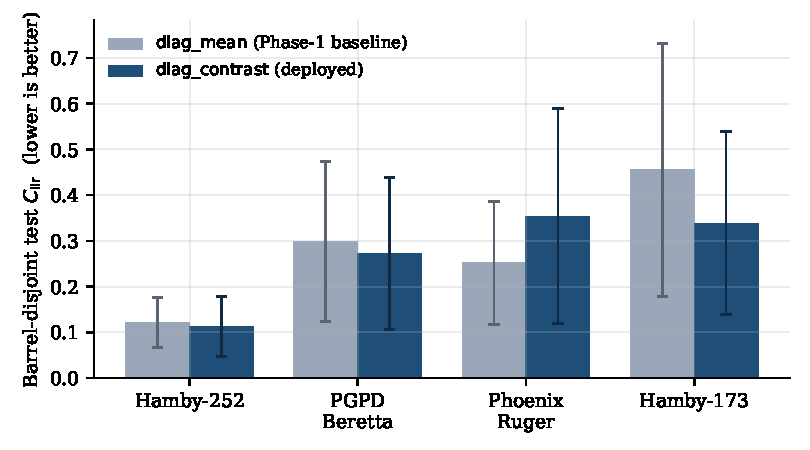
\includegraphics[width=0.78\linewidth]{fig_cllr_by_study.pdf}
  \caption{Barrel-disjoint test $\Cllr$ per study, baseline (\diagmean) vs deployed
    (\diagcontrast); error bars are the cross-fold standard deviation. Generated
    from \code{data/ablation.json}. The wide error bars on the smaller NBTRD sets
    are the honest signature of limited source-disjoint data.}
  \label{fig:cllr}
\end{figure}

\subsection{Scorer selection by ablation}
\label{sec:scorerablation}
The choice of \diagcontrast{} as the production scorer was made \emph{by the data},
not assumed. We ran a barrel-disjoint ablation over the candidate scalars derived
from the CCF matrix --- the \diagmean{} baseline, \diagcontrast{}, the offset
margin, lag coherence, the weakest diagonal land --- and two multivariate fusions
of those features (a standardized logistic, and an isotonic fusion). The result is
a genuine rigor highlight, and it cuts against the reflex to add model capacity:

\begin{itemize}
  \item \diagcontrast{} beats the multivariate logistic fusion on three of the four
        studies, and has the lowest \emph{mean} barrel-disjoint $\Cllr$ across
        studies (Figure~\ref{fig:scorer}, Table~\ref{tab:scorer});
  \item the isotonic fusion --- the most flexible option --- \emph{overfits}: it has
        the worst mean source-disjoint $\Cllr$, despite the strongest in-sample
        discrimination;
  \item so the simple, single-number, fully interpretable \diagcontrast{} is the
        deployed scorer. A multivariate fusion remains available as an opt-in
        research path with two or three inspectable coefficients --- but it is not
        the default, because the data did not justify it.
\end{itemize}

\begin{table}[t]
  \centering
  \small
  \begin{tabular}{@{}lcccc@{}}
    \toprule
    \textbf{Scorer} & \textbf{Hamby-252} & \textbf{PGPD} & \textbf{Phoenix} & \textbf{Hamby-173} \\
    \midrule
    \diagmean{} (Phase-1)     & \num{0.121} & \num{0.299} & \num{0.252} & \num{0.456} \\
    \diagcontrast{} (deployed) & \num{0.113} & \num{0.273} & \num{0.354} & \num{0.338} \\
    fusion (logistic)         & \num{0.127} & \num{0.298} & \num{0.231} & \num{0.456} \\
    fusion (isotonic)         & \num{0.110} & \num{0.294} & \num{0.273} & \num{0.531} \\
    \bottomrule
  \end{tabular}
  \caption{Barrel-disjoint test $\Cllr$ by scorer and study (from
    \code{data/ablation.json}). \diagcontrast{} has the lowest cross-study mean
    (Fig.~\ref{fig:scorer}); the isotonic fusion's strong fit does not survive the
    source-disjoint split.}
  \label{tab:scorer}
\end{table}

\begin{figure}[t]
  \centering
  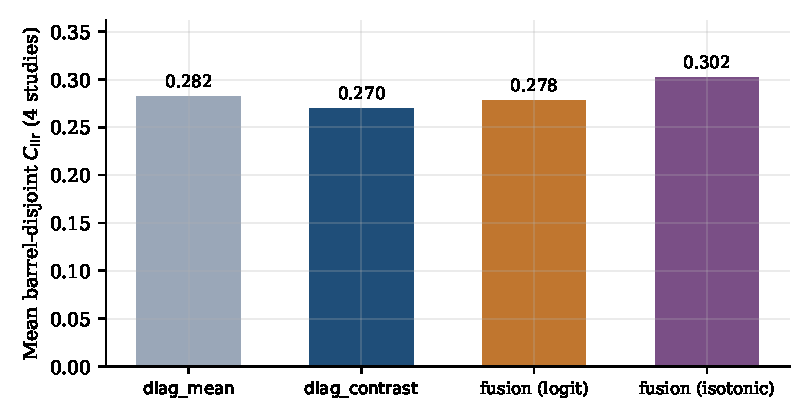
\includegraphics[width=0.72\linewidth]{fig_scorer_selection.pdf}
  \caption{Mean barrel-disjoint $\Cllr$ across the four bullet studies for each
    candidate scorer. \diagcontrast{} (deployed) is lowest; adding fusion capacity
    does not help on source-disjoint data, and the isotonic fusion is worst.}
  \label{fig:scorer}
\end{figure}

\paragraph{The pooled deployed reference.} For interactive use the deployed API
ships a pooled striated reference of $n_{\text{KM}}=146$ same-source and
$n_{\text{KNM}}=1755$ different-source land comparisons; on it the fitted system
reaches AUC $\approx \num{0.984}$, $\Cllr \approx \num{0.193}$, and
$\Cllrmin \approx \num{0.168}$ (pooling the four studies, including the harder
NBTRD sets, raises this above the per-study figures). This is an
\emph{in-sample} characterization of the bundled calibration and is labelled as
such; it is not a generalization claim. The generalization claims are the
barrel-disjoint numbers above.

\subsection{Closing the CMR table: cross-modality validation}
\label{sec:crossmodal}
Table~\ref{tab:cmr} is a \emph{claim}: one algorithm, three reductions. Here we
\emph{demonstrate} it. The same congruent-matching pipeline, under the \emph{same}
scorer configuration (one content hash shared across all three calibration
references), is validated source-disjoint on each modality
(Table~\ref{tab:reductions}). Every figure is recomputed from a committed reference by
the identical source-disjoint path used for bullets; the comparison baselines are
measured by a re-lockable harness (\S\ref{sec:platform}).

\begin{table}[t]
  \centering\small
  \begin{tabular}{@{}lllll@{}}
    \toprule
    \textbf{Reduction (modality)} & \textbf{Reference} & \textbf{Src-disjoint $\Cllr$} & \textbf{AUC} & \textbf{Baseline / specialist} \\
    \midrule
    Bullet lands (1-D striae)   & pooled, 4 studies   & $\num{0.186}\pm\num{0.126}$ & \num{0.989} & bulletxtrctr \num{0.064}; Hamby-252 alone \num{0.113} \\
    Cartridge breech (2-D)      & Fadul, 10 slides    & $\num{0.385}\pm\num{0.187}$ & \num{0.991} & cmcR \num{0.194}; areal \num{0.529} \\
    Screwdriver toolmark (1-D)  & \code{tmaRks}, 56 edges & $\num{0.328}\pm\num{0.050}$ & \num{0.957} & global align \num{0.447} \\
    \bottomrule
  \end{tabular}
  \caption{The CMR table, \emph{demonstrated}: one scorer configuration (shared config
    hash) reduced to each modality and validated source-disjoint ($\Cllr$ lower is
    better; mean $\pm$ SD over folds). Bullets are the pooled four-study reference
    (Hamby-252 alone is \num{0.113}); cartridges and toolmarks are their full sets. CMR
    matches or approaches the field-standard specialist in each case, and on toolmarks
    \emph{beats} the same-pipeline global baseline. From \code{data/cmr\_table.json} and
    \code{data/baselines.json}.}
  \label{tab:reductions}
\end{table}

\paragraph{Impressed (Fadul, CMR-2D).} The deployed 2-D reduction --- the same
\code{cmr\_count} consensus, now over 2-D cells under translation$+$rotation --- reaches
in-sample AUC \num{0.997} ($\Cllr\,\num{0.220}$, $\Cllrmin\,\num{0.070}$) and a
slide-disjoint $\Cllr$ of $\num{0.385}\pm\num{0.187}$ on the ten consecutively
manufactured Fadul slides. Figure~\ref{fig:cartridge} places it against the two
references on the \emph{same} slide-disjoint task: generic CMR-2D moves the naive global
areal cross-correlation (pooled AUC \num{0.911}, $\Cllr\,\num{0.529}$) most of the way
to the \code{cmcR} Congruent Matching Cells specialist~\cite{zemmels2023} (AUC \num{1.000},
$\Cllr\,\num{0.194}$) --- with no cartridge-specific engineering. CMR-2D instantiates
the same counting principle as CMC; the remaining gap to the tuned specialist
($\Cllr$ \num{0.385} vs \num{0.194}) is the measured price of keeping the
implementation generic, and closing it is ongoing work, not a claim already made.

\begin{figure}[t]
  \centering
  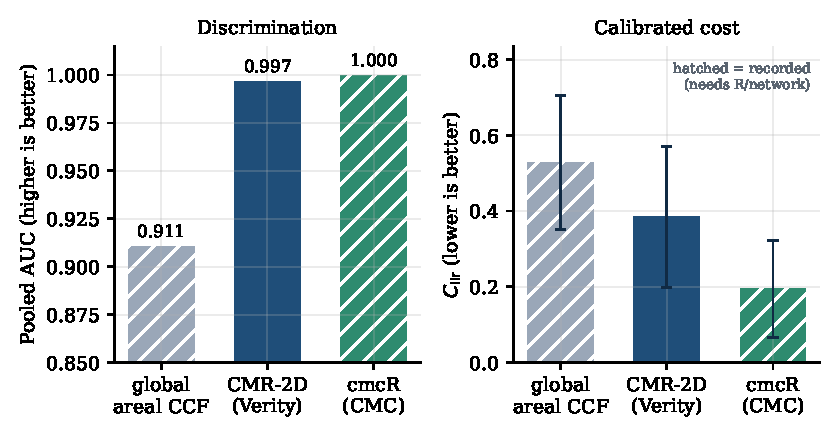
\includegraphics[width=0.82\linewidth]{fig_cllr_cartridge.pdf}
  \caption{Impressed-mark validation on the slide-disjoint Fadul task: the naive global
    areal CCF, the deployed generic CMR-2D, and the \code{cmcR} CMC specialist. Left:
    pooled AUC. Right: source-disjoint $\Cllr$ with cross-fold error bars. CMR-2D (solid;
    reproducible from the committed reference) lands beside the specialist; the baselines
    (hatched) need R to re-lock. Generated from \code{data/cartridge\_fadul.json} and
    \code{data/baselines.json}.}
  \label{fig:cartridge}
\end{figure}

\paragraph{Toolmarks (\code{tmaRks}, CMR-1D).} The 1-D reduction --- the
consecutive-striae statistic of Table~\ref{tab:cmr} --- is validated on the MIT
\code{tmaRks} consecutively-manufactured screwdriver set~\cite{tmarks} (580 marks
across 56 tool edges), source-disjoint by the mark-generating edge. (A flat-head
screwdriver carries two working edges; the split is disjoint by \emph{edge} --- the
mark generator --- so same-tool cross-edge pairs are treated as different-source.
The harness also supports tool-level-disjoint splits; locking that sensitivity
analysis is planned.) CMR-1D reaches AUC \num{0.957} at
$\Cllr\,\num{0.328}\pm\num{0.050}$ and, notably, \emph{beats} the same-pipeline global
1-D cross-correlation on the identical set (AUC \num{0.942}, $\Cllr\,\num{0.447}$):
requiring congruence among matching windows, rather than one global alignment, helps on
real toolmarks. This is a \emph{non-firearm} domain the pipeline was never tuned for ---
evidence the unification is not firearm-specific. (On the much smaller Ames Lab set, our run of the
\code{toolmaRk} $U$ statistic~\cite{hadler2018} gives pooled AUC \num{0.614} over 7
tools; with so few tools and replicates, that set is a weak benchmark for \emph{any}
method, which is why we report \code{tmaRks} as the primary toolmark benchmark.)

\paragraph{Reading these numbers.} The cross-modality $\Cllr$ values are larger than
Hamby-252's \num{0.113}, as they should be: cartridges and toolmarks have far fewer
sources (ten slides; the cross-edge toolmark task is genuinely hard), and the pooled
bullet reference mixes the harder NBTRD sets. The claim is not that every modality is as
strong as the best bullet study; it is that \emph{one calibrated algorithm, validated
source-disjoint, matches or approaches the field-standard method in each of the three
reductions of Table~\ref{tab:cmr}} --- Chumbley-style counting on toolmarks, CMC-style
counting on breech faces, and the bullet-land result --- rather than three bespoke
pipelines.

% ==========================================================================
\section{Limitations and honest scope}
\label{sec:limits}

We would rather state the boundaries plainly than have a reviewer find them.

\begin{itemize}
  \item \textbf{Model selection used the validation studies; no untouched
        confirmation set exists yet.} The deployed scorer (\diagcontrast), the
        FFT orientation front-end (\S\ref{sec:region}), and the filter cutoffs
        were chosen by barrel-disjoint ablations on the \emph{same} four bullet
        studies reported in \S\ref{sec:validation}. Each fold is honest --- the
        calibration never sees a held-out source --- but repeated evaluation
        against the same source-disjoint splits during development means the
        headline numbers are best read as \emph{development-set performance under
        a source-disjoint protocol}, not as a one-shot confirmation on new data.
        This is the same selection-leakage failure mode Cuellar et
        al.~\cite{cuellar2024} flag in black-box studies, and it applies to us
        until a confirmation set is run. The frozen open-benchmark splits commit
        the protocol going forward; a one-shot validation on data never used in
        development (new NBTRD collections; the LAPD corpus) is the next
        validation milestone.
  \item \textbf{Small source-disjoint sets widen uncertainty.} Consecutively
        manufactured benchmarks are small in the dimension that matters --- sources.
        Fadul has $\approx\!10$ slides; the bullet sets have 8--10 barrels. With so
        few held-out sources the fold-to-fold $\Cllr$ has a large standard deviation
        (Fig.~\ref{fig:cllr}), and the empirical LR cap (Eq.~\ref{eq:elub}) is
        correspondingly low. More independent sources would tighten both.
  \item \textbf{Score-based LR limitations.} As in \S\ref{sec:calibration}, the
        reported LR is a property of the score and the named reference, not an
        unconditional weight of evidence~\cite{hepler2012,neumann2020}; a reference
        unrepresentative of a casework population would mis-calibrate, which is why
        the scope guard exists.
  \item \textbf{Not a universal error rate.} Nothing here should be read as ``the
        error rate of firearms identification.'' Every number is conditioned on a
        named population and a stated protocol. This is the intended reading of our
        answer to Cuellar et al., not a hedge.
  \item \textbf{The learned representation does not yet beat the baseline.} A
        Phase-2b learned (embedding) representation is implemented behind the same
        firewall, but on the data available it does not yet outperform the
        cross-correlation baseline. We treat this as a data limitation, not a
        success, and the deployed system uses the interpretable baseline. The concrete
        path is self-supervised pretraining on the unlabelled LAPD ($\approx\!15$k-scan)
        corpus, fine-tuned behind the same firewall and retested barrel-disjoint --- an
        orthogonal research track, not a precondition for the calibrated-LR results above.
  \item \textbf{The cross-modality reductions rest on few sources.} The impressed
        (Fadul, $\approx\!10$ slides) and toolmark (\code{tmaRks}) reductions are now
        demonstrated source-disjoint (\S\ref{sec:crossmodal}) --- and CMR-1D even beats
        the same-pipeline global baseline on toolmarks --- but with far fewer independent
        sources than the bullet benchmarks, so the wider $\Cllr$ and low LR caps
        reflect that. They are a genuine cross-modality demonstration of the CMR
        unification, not yet a definitive per-modality error characterization.
\end{itemize}

% ==========================================================================
\section{The platform}
\label{sec:platform}

The methods above are only useful in court and in the lab if they are reproducible,
fast, and inspectable. Verity is built as production software, not a script.

\begin{itemize}
  \item \textbf{Native Rust X3P codec.} A from-scratch reader/writer for the
        ISO~25178-72 / ISO~5436-2 X3P format (\code{crates/verity-x3p}), with
        Python and R bindings. It interoperates with the reference \code{x3ptools}
        R reader~\cite{x3ptools2024} but removes the heavy runtime dependency,
        giving fast, portable scan I/O for both research and deployment.
  \item \textbf{A calibrated-LR REST API.} A deployed service exposes \code{/detect}
        (suggest a mark type from a scan), \code{/compare} (return the calibrated,
        bounded LR with its bootstrap interval and the region attribution), and a
        \code{/health} endpoint that publishes the currently calibrated domains ---
        the scope guard, machine-readable.
  \item \textbf{A local-first data catalog.} A catalog service harvests and labels
        the open NBTRD~\cite{nbtrd2020} 3-D scans --- which have no public API ---
        succeeding the earlier CSAFE scraper (unmaintained since 2020) with a
        maintained, reproducible harvester, alongside the Fadul and \code{tmaRks}
        sets, so validation runs against versioned, content-addressed, reproducible
        data.
  \item \textbf{An open, frozen benchmark.} Frozen source-disjoint splits
        (bullets, cartridge, toolmark) with published split hashes, a downloadable
        replication kit whose offline scorer matches the server exactly, and a
        public leaderboard ranked by total $\Cllr$. The leaderboard protocol
        scores one LR per pair via a single leave-the-pair's-sources-out
        calibration, which differs from the per-fold refits reported above ---
        e.g.\ Fadul source-disjoint $\Cllr$ is \num{0.385} under
        \S\ref{sec:crossmodal}'s protocol and \num{0.398} on the leaderboard. Both
        are source-disjoint; the kit reproduces the leaderboard numbers exactly.
  \item \textbf{Reproducible validation reports.} Every number in
        \S\ref{sec:validation} is recomputed from a committed calibration reference by a
        checked-in harness and persisted as the paper's source of truth:
        \code{data/ablation.json} (bullets), \code{data/cmr\_table.json} (the three
        reductions), \code{data/cartridge\_fadul.json}, \code{data/toolmark\_tmaRks.json},
        and \code{data/baselines.json} (the comparison baselines, re-lockable offline via
        \code{verity-relock-baselines}); the figures are regenerated from those files by a
        checked-in script.
\end{itemize}

\paragraph{An invitation.} Verity is the production, calibration, and validation
layer for a research program it did not invent. The natural next step is to validate
it on larger, more representative, genuinely source-disjoint reference collections
--- the kind of data the CSAFE program is built to produce. We offer the codec, the
calibration firewall, and the validation harness as open infrastructure, and we
would welcome a collaboration that puts a properly powered reference behind the
calibrated LR. That is a proposal, not a claim of endorsement.

% ==========================================================================
\section*{Acknowledgments}
\addcontentsline{toc}{section}{Acknowledgments}
Verity stands entirely on the CSAFE / Iowa State research program and the NIST
congruent-matching line: the bullet-matching method of Hare, Hofmann \&
Carriquiry~\cite{hare2017}, the \code{bulletxtrctr} pipeline and similarity-score
study of Vanderplas et al.~\cite{vanderplas2020}, the Congruent Matching Cells
method of Song and colleagues~\cite{song2013,song2018}, the Chumbley
toolmark statistic~\cite{chumbley2010}, the \code{x3ptools} format
tooling~\cite{x3ptools2024}, the open benchmark data~\cite{hamby2009,fadul2011,nbtrd2020},
and the calibration metric of Br\"ummer \& du Preez~\cite{brummer2006}. Mention of
CSAFE denotes intellectual lineage and a prospective collaboration only; it does
not imply review or endorsement of Verity by CSAFE, Iowa State University, NIST, or
any author of the cited works.

% ==========================================================================
% A dependency-free thebibliography so the paper builds anywhere (no bibtex run).
\begin{thebibliography}{99}
\small

\bibitem{hare2017} E.~Hare, H.~Hofmann \& A.~Carriquiry (2017).
  Automatic matching of bullet land impressions. \emph{The Annals of Applied
  Statistics} \textbf{11}(4), 2332--2356. \href{https://doi.org/10.1214/17-AOAS1080}{doi:10.1214/17-AOAS1080}.

\bibitem{song2013} J.~Song (2013). Proposed congruent matching cells (CMC) method
  for ballistic identification and error rate estimation. \emph{AFTE Journal}
  \textbf{45}(2), 184--194. NIST.

\bibitem{song2018} J.~Song, T.~V.~Vorburger, W.~Chu, J.~Yen, J.~A.~Soons,
  D.~B.~Ott \& N.~F.~Zhang (2018). Estimating error rates for firearm evidence
  identifications in forensic science. \emph{Forensic Science International}
  \textbf{284}, 15--32. \href{https://doi.org/10.1016/j.forsciint.2017.12.013}{doi:10.1016/j.forsciint.2017.12.013}.

\bibitem{chumbley2010} L.~S.~Chumbley, M.~D.~Morris, M.~J.~Kreiser, C.~Fisher,
  J.~Craft, L.~J.~Genalo, S.~Davis, D.~Faden \& J.~Kidd (2010). Validation of tool
  mark comparisons obtained using a quantitative, comparative, statistical
  algorithm. \emph{Journal of Forensic Sciences} \textbf{55}(4), 953--961.
  \href{https://doi.org/10.1111/j.1556-4029.2010.01424.x}{doi:10.1111/j.1556-4029.2010.01424.x}.

\bibitem{nrc2009} National Research Council (2009). \emph{Strengthening Forensic
  Science in the United States: A Path Forward}. The National Academies Press.
  \href{https://doi.org/10.17226/12589}{doi:10.17226/12589}.

\bibitem{pcast2016} President's Council of Advisors on Science and Technology
  (2016). \emph{Forensic Science in Criminal Courts: Ensuring Scientific Validity
  of Feature-Comparison Methods}. Executive Office of the President.

\bibitem{cuellar2024} M.~Cuellar, S.~Vanderplas, A.~Luby \& M.~Rosenblum (2024).
  Methodological problems in every black-box study of forensic firearm
  comparisons. \emph{Law, Probability and Risk} \textbf{23}(1), mgae015.
  \href{https://doi.org/10.1093/lpr/mgae015}{doi:10.1093/lpr/mgae015}.

\bibitem{hamby2009} J.~E.~Hamby, D.~J.~Brundage \& J.~W.~Thorpe (2009). The
  identification of bullets fired from 10 consecutively rifled 9\,mm Ruger pistol
  barrels: a research project involving 507 participants from 20 countries.
  \emph{AFTE Journal} \textbf{41}(2), 99--110.

\bibitem{fadul2011} T.~G.~Fadul, G.~A.~Hernandez, S.~Stoiloff \& S.~Gulati (2011).
  An empirical study to improve the scientific foundation of forensic firearm and
  tool mark identification utilizing 10 consecutively manufactured slides.
  \emph{AFTE Journal} \textbf{43}(3). NIJ Award 2009-DN-BX-K230.

\bibitem{nbtrd2020} X.~Zheng, J.~Soons, T.~V.~Vorburger et al.\ (NIST) (2020).
  NIST Ballistics Toolmark Research Database. \emph{Journal of Research of NIST}
  \textbf{125}, 125004. \href{https://doi.org/10.6028/jres.125.004}{doi:10.6028/jres.125.004}.

\bibitem{x3ptools2024} H.~Hofmann, S.~Vanderplas, G.~Krishnan \& E.~Hare (2024).
  x3ptools: Tools for Working with 3D Surface Measurements. R package (CRAN),
  v0.0.4. \href{https://doi.org/10.32614/CRAN.package.x3ptools}{doi:10.32614/CRAN.package.x3ptools}.

\bibitem{vanderplas2020} S.~Vanderplas, M.~Nally, T.~Klep, C.~Cadevall \&
  H.~Hofmann (2020). Comparison of three similarity scores for bullet LEA
  matching. \emph{Forensic Science International} \textbf{308}, 110167.
  \href{https://doi.org/10.1016/j.forsciint.2020.110167}{doi:10.1016/j.forsciint.2020.110167}.

\bibitem{brummer2006} N.~Br\"ummer \& J.~du Preez (2006). Application-independent
  evaluation of speaker detection. \emph{Computer Speech \& Language}
  \textbf{20}(2--3), 230--275. \href{https://doi.org/10.1016/j.csl.2005.08.001}{doi:10.1016/j.csl.2005.08.001}.

\bibitem{hepler2012} A.~B.~Hepler, C.~P.~Saunders, L.~J.~Davis \& J.~Buscaglia
  (2012). Score-based likelihood ratios for handwriting evidence. \emph{Forensic
  Science International} \textbf{219}(1--3), 129--140.
  \href{https://doi.org/10.1016/j.forsciint.2011.12.009}{doi:10.1016/j.forsciint.2011.12.009}.
\bibitem{neumann2020} C.~Neumann \& M.~Ausdemore (2020). Defence against the modern
  arts: the curse of statistics --- Part II: ``Score-based likelihood ratios''.
  \emph{Law, Probability and Risk} \textbf{19}(1), 21--42.
  \href{https://doi.org/10.1093/lpr/mgaa006}{doi:10.1093/lpr/mgaa006}.
\bibitem{vergeer2016} P.~Vergeer, A.~van Es, A.~de Jongh, I.~Alberink \& R.~Stoel
  (2016). Numerical likelihood ratios outputted by LR systems are often based on
  extrapolation: when to stop extrapolating? \emph{Science \& Justice}
  \textbf{56}(6), 482--491.
  \href{https://doi.org/10.1016/j.scijus.2016.06.003}{doi:10.1016/j.scijus.2016.06.003}.
  {\footnotesize (Empirical-bound / ELUB principle.)}

\bibitem{zemmels2023} J.~Zemmels, S.~Vanderplas \& H.~Hofmann (2023). A study in
  reproducibility: the congruent matching cells algorithm and \code{cmcR} package.
  \emph{The R Journal} \textbf{14}(4), 79--102.
  \href{https://journal.r-project.org/articles/RJ-2023-014/}{RJ-2023-014}.

\bibitem{hadler2018} J.~R.~Hadler \& M.~D.~Morris (2018). An improved version of
  a tool mark comparison algorithm. \emph{Journal of Forensic Sciences}
  \textbf{63}(3), 849--855. {\footnotesize (Implemented in the \code{toolmaRk} R
  package.)}

\bibitem{krishnan2019} G.~Krishnan \& H.~Hofmann (2019). Adapting the Chumbley
  score to match striae on land engraved areas (LEAs) of bullets. \emph{Journal of
  Forensic Sciences} \textbf{64}(3), 728--740.
  \href{https://doi.org/10.1111/1556-4029.13950}{doi:10.1111/1556-4029.13950}.

\bibitem{tai2018} X.~H.~Tai \& W.~F.~Eddy (2018). A fully automatic method for
  comparing cartridge case images. \emph{Journal of Forensic Sciences}
  \textbf{63}(2), 440--448.
  \href{https://doi.org/10.1111/1556-4029.13577}{doi:10.1111/1556-4029.13577}.

\bibitem{morrison2013} G.~S.~Morrison (2013). Tutorial on logistic-regression
  calibration and fusion: converting a score to a likelihood ratio.
  \emph{Australian Journal of Forensic Sciences} \textbf{45}(2), 173--197.
  \href{https://doi.org/10.1080/00450618.2012.733025}{doi:10.1080/00450618.2012.733025}.

\bibitem{meuwly2017} D.~Meuwly, D.~Ramos \& R.~Haraksim (2017). A guideline for
  the validation of likelihood ratio methods used for forensic evidence
  evaluation. \emph{Forensic Science International} \textbf{276}, 142--153.
  \href{https://doi.org/10.1016/j.forsciint.2016.03.048}{doi:10.1016/j.forsciint.2016.03.048}.

\bibitem{enfsi2015} S.~M.~Willis et al.\ (2015). \emph{ENFSI Guideline for
  Evaluative Reporting in Forensic Science} (Strengthening the Evaluation of
  Forensic Results across Europe, v3.0). European Network of Forensic Science
  Institutes.
  \href{https://enfsi.eu/wp-content/uploads/2016/09/m1_guideline.pdf}{enfsi.eu}.

\bibitem{tmarks} M.~Cuellar, S.~Gao \& H.~Hofmann (2024). An algorithm for
  forensic toolmark comparisons. \emph{Forensic Science International: Synergy}.
  \href{https://arxiv.org/abs/2312.00032}{arXiv:2312.00032}. Data: the
  \code{tmaRks} consecutively-manufactured screwdriver toolmark scans,
  \href{https://github.com/heike/tmaRks}{github.com/heike/tmaRks} (MIT license).

\end{thebibliography}

\end{document}
